% The first two PDFs have 10-pt labels and 9-pt ticks at 3-inch width.
% Include at approximately half of the 6-inch text width; do not shrink further.
\begin{figure}[t]
    \centering
    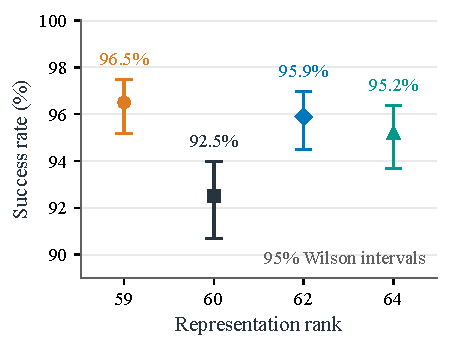
\includegraphics[width=0.49\linewidth]{figures/reacher_rank_1000/rank_success_rate.pdf}\hfill
    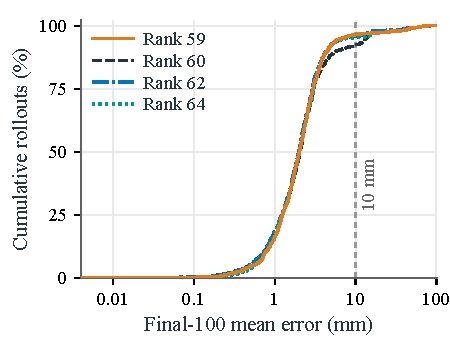
\includegraphics[width=0.49\linewidth]{figures/reacher_rank_1000/rank_tracking_error.pdf}
    \caption{Rank sensitivity over the same 1,000 seeds (311--1310). Left: success rates with pointwise 95\% Wilson intervals. Success requires mean error below 10\,mm and maximum error below 20\,mm in both the final-30 and final-100 windows. Right: empirical distributions of final-100 mean fingertip error, including failed rollouts. The 10\,mm line marks only the mean-error component of the success criterion.}
    \label{fig:rank-performance}
\end{figure}

\begin{figure}[t]
    \centering
    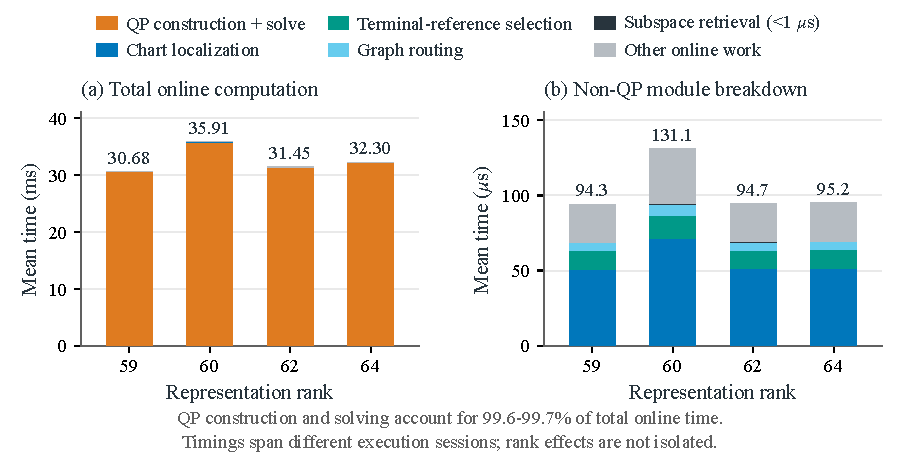
\includegraphics[width=\linewidth]{figures/reacher_rank_1000/rank_module_timing.pdf}
    \caption{Mean online computation time: (a) total module costs in milliseconds and (b) the non-QP components on an expanded microsecond scale. Each rank includes 315,000 timed steps after excluding the first five steps of each rollout. QP time includes construction and solving; offline computation and one-time reference setup are excluded. Measurements span different sessions on a shared computer and do not isolate the effect of rank on runtime.}
    \label{fig:rank-timing}
\end{figure}
